\documentclass[a4paper, 10pt]{article}
\usepackage{standart-header}
\fancyhead[R]{Viner Daniil. BEDA232}
\fancyfoot [C] {\thepage}
\usepackage{pgfplots}
\setlength{\parindent}{15pt}
\setlength{\parskip}{2mm}
\fancyhead[L]{Microeconomics—1. Seminar—1 06.09.2024}

\begin{document}
\section*{Problem №1}
The cost function of a non-discriminating monopolist is $c(y)=y^2+12$, and the inverse demand function is $p(y)=24-y$.
\subsection*{Subproblem №1}
From Micro—1 we remember, that $MR=TR'$ and $TR=p(y)\cdot y$. So, let's calculate
\begin{equation*}
    MR=TR'=(p(y)y)'=(24y-y^2)'=24-2y
\end{equation*}

As we know, $MR=MC$. Moreover, $MC=c'(y)=2y$. Logically:
\begin{equation*}
    \begin{aligned}
        24-2y&=2y\\
        y^*&=6\text{ — optimal $y$, then}\\
        p^*&=p(6)=18\text{ — optimal price}
    \end{aligned}
\end{equation*}

Let's put that equilibrium price and output into profit function:
\begin{equation*}
    \Pi=\underbrace{24\cdot6-36}_{TR}-\underbrace{36-12}_{c}=60
\end{equation*}

\subsection*{Subproblem №2}
% It's obvious where is $CS,PS$ and $DWL$ on the graphic
\textcolor{green}{$CS$}, \textcolor{blue}{$PS$} and \textcolor{black}{$DWL$} can be computed as squares of figures shown below
$$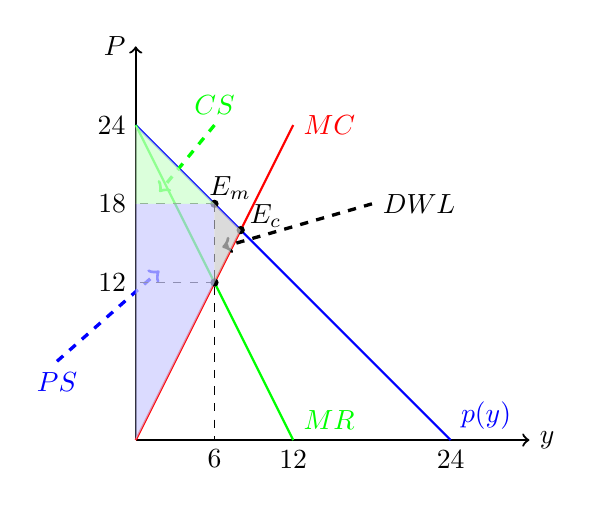
\begin{tikzpicture}
    \draw[thick,->] (0,0) -- (0, 5) node[left] {$P$};
    \draw[thick, ->] (0,0) -- (5,0) node[right] {$y$};
    \draw[thick, blue] (0,4) node[left, black] {$24$} -- (4,0) node[below, black] {$24$} node[above right, blue] {$p(y)$}; %p(y)
    \draw[thick, green] (0,4) -- (2,0) node[below, black] {$12$} node[above right, green] {$MR$}; %MR
    \draw[thick, red] (0,0) -- (2,4) node[right, red] {$MC$}; %MC

    \draw[dashed, very thick, green, ->] (1,4) node[above, green] {$CS$} -- (0.3,3.15);
    \draw[dashed, very thick, blue, ->] (-1,1) node[below, blue] {$PS$} -- (0.3,2.15);
    \draw[dashed, very thick, black, ->] (3,3) node[right, black] {$DWL$} -- (1.1,2.45);

    \draw[dashed, black] (1,3) -- (1,0) node[below] {$6$};
    \draw[dashed, black] (1,2)--(0,2) node[left] {$12$};
    \draw[dashed, black] (1,3)--(0,3) node[left] {$18$};

    \fill[black] (1,3) circle (1.5pt);
    \node[black] at (1.2,3.2) {$E_m$};

    \fill[black] (1.33333, 2.66667) circle (1.5pt);
    \node[black] at (1.65, 2.84) {$E_c$};

    \fill[black] (1,2) circle (1.5pt);

    \fill[fill=green!20,opacity=0.7] 
        (0, 4) -- (0,3) -- (1,3) -- cycle;

    \fill[fill=blue!20,opacity=0.7] 
        (0, 0) -- (1,2) -- (1,3) -- (0,3) -- cycle;

    \fill[fill=black!20,opacity=0.7] 
        (1,2) -- (1.33333, 2.66667) -- (1,3) -- cycle;
    
    
\end{tikzpicture}$$

Moreover, in the picture we illustrated answers on \textbf{Subproblem №1}

$CS=\displaystyle\frac{(24-18)\cdot6}{2}=18$

$PS=\displaystyle\frac{18+6}{2}\cdot6=72$

$DWL=\displaystyle\frac{6\cdot2}{2}=6$

\subsection*{Subproblem №3}
$$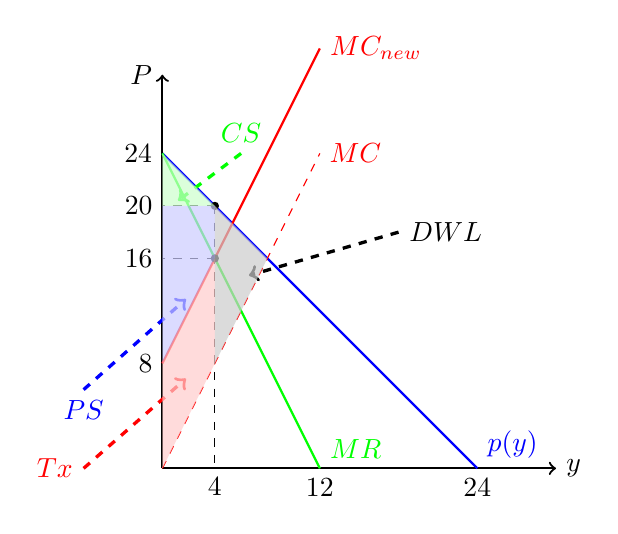
\begin{tikzpicture}
    \draw[thick,->] (0,0) -- (0, 5) node[left] {$P$};
    \draw[thick, ->] (0,0) -- (5,0) node[right] {$y$};
    \draw[thick, blue] (0,4) node[left, black] {$24$} -- (4,0) node[below, black] {$24$} node[above right, blue] {$p(y)$}; %p(y)
    \draw[thick, green] (0,4) -- (2,0) node[below, black] {$12$} node[above right, green] {$MR$}; %MR
    \draw[dashed, red] (0,0) -- (2,4) node[right, red] {$MC$}; %MC
    \draw[thick, red] (0,1.33333) -- (2,5.33333) node[right, red] {$MC_{new}$}; %MC

    \draw[dashed, very thick, green, ->] (1,4) node[above, green] {$CS$} -- (0.2,3.4);
    \draw[dashed, very thick, blue, ->] (-1,1) node[below, blue] {$PS$} -- (0.3,2.15);
    \draw[dashed, very thick, black, ->] (3,3) node[right, black] {$DWL$} -- (1.1,2.45);
    \draw[dashed, very thick, red, ->] (-1,0) node[left, red] {$Tx$} -- (0.3,1.14);

    \draw[dashed, black] (0.66667, 3.33333) -- (0.66667, 0) node[below] {$4$};
    \draw[dashed, black] (0.66667, 2.66667)--(0, 2.66667) node[left] {$16$};
    \draw[dashed, black] (0.66667, 3.33333)--(0, 3.33333) node[left] {$20$};

    \node[black, left] at (0,1.33333) {$8$};
    % \fill[black] (1,3) circle (1.5pt);
    % \node[black] at (1.2,3.2) {$E_m$};

    % \fill[black] (1.33333, 2.66667) circle (1.5pt);
    % \node[black] at (1.65, 2.84) {$E_c$};

    \fill[black] (0.66667, 2.66667) circle (1.5pt);
    \fill[black] (0.66667, 3.33333) circle (1.5pt);

    \fill[fill=green!20,opacity=0.7] 
        (0, 4) -- (0,3.33333) -- (0.66667, 3.33333) -- cycle;

    \fill[fill=blue!20,opacity=0.7] 
        (0, 1.33333) -- (0.66667, 2.66667) -- (0.66667, 3.33333) -- (0,3.33333) -- cycle;

    \fill[fill=red!20,opacity=0.7] 
        (0, 0) -- (0.66667, 1.33333) -- (0.66667, 2.66667) -- (0,1.33333) -- cycle;

    \fill[fill=black!20,opacity=0.7] 
        (0.66667, 1.33333) -- (1.33333, 2.66667) -- (0.66667, 3.33333) -- cycle;
    
    
\end{tikzpicture}$$

$\begin{aligned}
    MC_{new}=MR\Longrightarrow2y+8=24-2y\Longrightarrow y^*=4,\ p^*=20
\end{aligned}$

$CS_{new}=4\cdot4\cdot\displaystyle\frac{1}{2}=8$

$PS_{new}=\displaystyle\frac{1}{2}\cdot(12+4)\cdot4=32$

$DWL_{new}=\displaystyle\frac{1}{2}\cdot4\cdot12=24$

$SW=CS_{new}+PS_{new}+Tx=8+32+8=48$

$Tx=\text{quantity $\cdot$ tax}=4\cdot8=32$

\subsection*{Subproblem №4}
Basic profit formula: $\Pi=p(y)\cdot y-c(y)$

In our constraints it'll be like $$\Pi=24y-y^2-y^2-12$$

Imagine that government created some income tax $t$, our progit formula will transform into:
\begin{equation*}
    \Pi=\underbrace{(1-t)(24y-y^2)}_{TR_{\text{new}}}-\underbrace{(1-t)(y^2+12)}_{TC_{\text{new}}}
\end{equation*}

Let's calculate $MR_4$ and $MC_4$%\footnote{$4$ means the number of subproblem}:
\begin{equation*}
    \begin{cases}
        MR_4=((1-t)((24-y)y))^{\prime}=(1-t)(24-2y)\\
        MC_4=(1-t)2y
    \end{cases}\Longrightarrow\begin{cases}
        y^*=6\\
        p^*=p(y^*)=18
    \end{cases}
\end{equation*}

It means, that $\Pi=18\cdot6\cdot(1-t)\Longrightarrow\text{ profit is less than without taxes}$

$$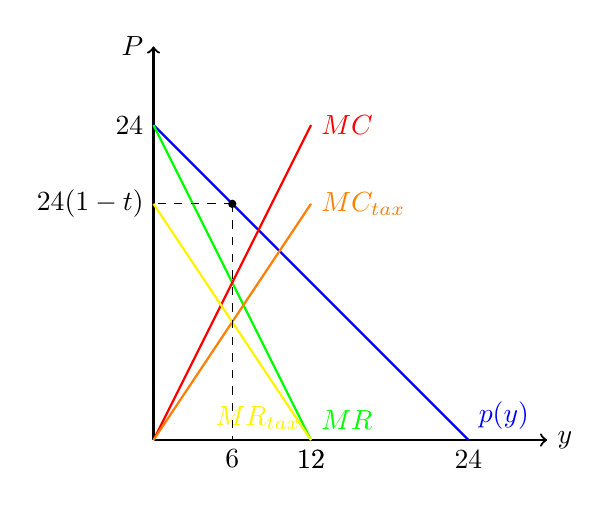
\begin{tikzpicture}
    \draw[thick,->] (0,0) -- (0, 5) node[left] {$P$};
    \draw[thick, ->] (0,0) -- (5,0) node[right] {$y$};
    \draw[thick, blue] (0,4) node[left, black] {$24$} -- (4,0) node[below, black] {$24$} node[above right, blue] {$p(y)$}; %p(y)
    \draw[thick, green] (0,4) -- (2,0) node[below, black] {$12$} node[above right, green] {$MR$}; %MR
    \draw[thick, red] (0,0) -- (2,4) node[right, red] {$MC$}; %MC
    \draw[thick, orange] (0,0) -- (2,3) node[right, orange] {$MC_{tax}$};
    \draw[thick, yellow] (0,3) -- (2,0) node[above left, yellow] {$MR_{tax}$} node[below, black] {$12$}; %MR
    % \draw[thick, red] (0,1.33333) -- (2,5.33333) node[right, red] {$MC_{new}$}; %MC

    % \draw[dashed, very thick, green, ->] (1,4) node[above, green] {$CS$} -- (0.2,3.4);
    % \draw[dashed, very thick, blue, ->] (-1,1) node[below, blue] {$PS$} -- (0.3,2.15);
    % \draw[dashed, very thick, black, ->] (3,3) node[right, black] {$DWL$} -- (1.1,2.45);
    % \draw[dashed, very thick, red, ->] (-1,0) node[left, red] {$Tx$} -- (0.3,1.14);

    \draw[dashed, black] (1,3) -- (1,0) node[below] {$6$};
    \draw[dashed, black] (1,3)--(0,3) node[left] {$24(1-t)$};
    % \draw[dashed, black] (0.66667, 3.33333)--(0, 3.33333) node[left] {$20$};

    % \node[black, left] at (0,1.33333) {$8$};
    \fill[black] (1,3) circle (1.5pt);
    % \node[black] at (1.2,3.2) {$E_m$};

    % \fill[black] (1.33333, 2.66667) circle (1.5pt);
    % \node[black] at (1.65, 2.84) {$E_c$};

    % \fill[black] (0.66667, 2.66667) circle (1.5pt);
    % \fill[black] (0.66667, 3.33333) circle (1.5pt);

    % \fill[fill=green!20,opacity=0.7] 
    %     (0, 4) -- (0,3.33333) -- (0.66667, 3.33333) -- cycle;

    % \fill[fill=blue!20,opacity=0.7] 
    %     (0, 1.33333) -- (0.66667, 2.66667) -- (0.66667, 3.33333) -- (0,3.33333) -- cycle;

    % \fill[fill=red!20,opacity=0.7] 
    %     (0, 0) -- (0.66667, 1.33333) -- (0.66667, 2.66667) -- (0,1.33333) -- cycle;

    % \fill[fill=black!20,opacity=0.7] 
    %     (0.66667, 1.33333) -- (1.33333, 2.66667) -- (0.66667, 3.33333) -- cycle;
    
    
\end{tikzpicture}$$

Significantly, that in monopoly with income taxes optimal keeps the same as in previous subproblems

$MR_{tax}^{\prime}=0=(1-t)(24-2y)\Longrightarrow y^*=12$

$Tx=60\cdot t$

$PS_4=TR-VC=\Pi+FC=60(1-t)+12(1-t)$

\begin{equation*}
    \begin{cases}
        SW_{\text{in this monopoly}}&=90-12t\\
        SW_{\text{perfect comp}}&=96
    \end{cases}\Longrightarrow DWL=6+12t
\end{equation*}

\section*{Problem №2}
A monopolist uses technology with a cost function $c(y)=\frac{5}{3}y^2$ and can sell his product in two regions, price discrimination between which is prohibited.  The inverse function of demand for monopoly goods in the first region is $p_1 = 10- y_1$, and in the second region $p_2 = 13- 0.5y_2$

\subsection*{Subproblem №1}
$$\begin{tikzpicture}
    \draw[thick,->] (0,0) -- (0,4) node[left] {$P$};
    \draw[thick, ->] (0,0) -- (7,0) node[right] {$y$};
    \draw[thick, blue] (0,3) node[left, black] {$13$} -- (1,2);
    \draw[thick, red] (1,2) -- (6,0);
    \draw[dashed, black] (0,2) node[left, black] {$10$} -- (7,2);
    \draw[dashed, black] (0,3) -- (7,3);

\end{tikzpicture}$$
$y_1=\begin{cases}
    10-p_1,\ p_1\leqslant10\\
    0,\ p>10
\end{cases},\ y_2=\begin{cases}
    26-2p_2,\ p_1\leqslant13\\
    0,\ p>13
\end{cases}\Longrightarrow y_1+y_2=\begin{cases}
    36-3p,\ p\leqslant10\\
    26-2p,\ p\in(10,13)\\
    0,\ p>13
\end{cases}$

From the system of $(y_1+y_2)$ we'll find $p^*$:
\begin{equation*}
    p^*=\begin{cases}
    12 - \frac{y}{3},\ y\in \left[0,6\right] \\
    13-\frac{y}{2},\ y\in \left(6,36\right]
\end{cases}
\end{equation*}

\begin{equation*}
    \Pi=\begin{cases}
        13y-0.5y^2-\displaystyle\frac{5}{3}y^2,\ y\in\left[0,6\right]\\
        12y-\displaystyle\frac{y^2}{3}-\frac{5}{3}y^2,\ y\in\left(6,36\right]
    \end{cases}
\end{equation*}

If we analyze this profit, we'll realize that after $y=6$ the graphic will be under horizontal line that's why we don't need to draw it and take into consideration

So, we analyze the first equation. It's a parabola, branches down, so the maximum will be in the top. Skip simple calculations and we get optimal price and quantity:
\begin{equation*}
    \begin{cases}
        y^*=3\\
        p^*=p(y^*)=12
    \end{cases}
\end{equation*}

Another subproblems will be solved on the next seminar





\end{document}
